\section{Magnetospheric Magnetohydrodynamics}
\subsection{Earth's Magnetosphere}

\begin{frame}
\frametitle{Earth's Magnetosphere}
\begin{figure}
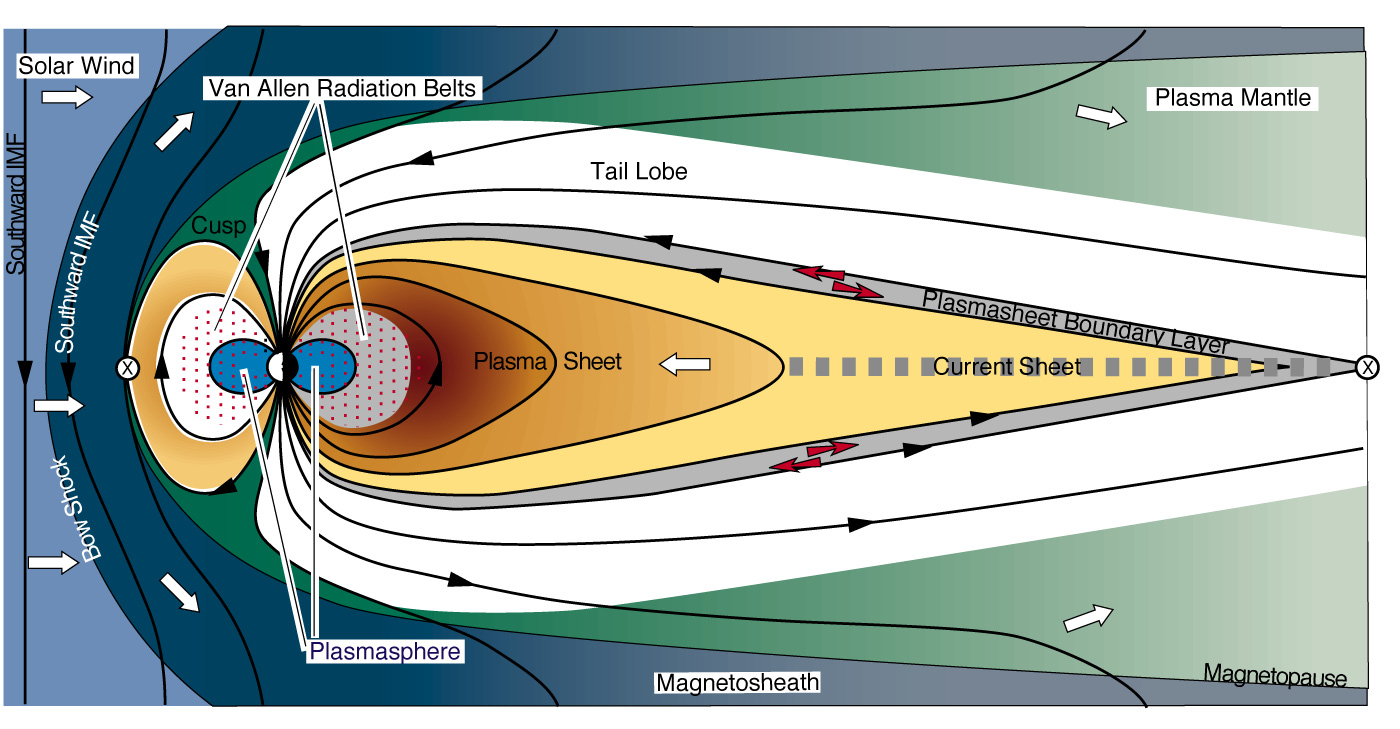
\includegraphics[scale=0.21]{images/Rice_Magnetosphere.jpg}
\end{figure}

\begin{itemize}
  \item Shape determined from a balance between kinetic pressure from the solar
  wind and magnetic pressure from Earth's magnetic field.
  \item IMF direction has most influence on magnetospheric response.
  \item Fluctuates between a bell and teardrop shape.
  \item Reconnection most supported theory for energy transfer in magnetosphere.
\end{itemize}

\end{frame}

\subsection{Magnetohydrodynamics}

\begin{frame}[shrink]
\frametitle{Magnetohydrodynamics}
\begin{tabular}{p{0.5\textwidth}p{0.5\textwidth}}
\begin{itemize}
  \item[] \textbf{Magnetohydrodynamics}
  \item Start with Boltzmann equation for single species.
  \item Invoke conservation of Mass, Momentum, Energy.
  \item Conservation equations summed over all species, treated as a single
  fluid.
  \item Use Maxwell's Equations:
  \begin{itemize}
    \item Gauss' Law.
    \item Gauss' Law for Magnetism.
    \item Faraday's Law.
    \item Ampere's Law.
  \end{itemize}
  
\end{itemize}
 &
\begin{itemize}
  \item[] \textbf{Ideal MHD}
  \item The time derivative of E is small
  \item Isotropic Pressure
  \item Charge neutrality
  \item Neglect small terms
  \item Single ion flow with collision term approximation
  \item Perfect conductivity
\end{itemize}

\begin{itemize}
  \item[] \textbf{Implementation}
  \item Grid Choice
  \item Discretization
\end{itemize}
\end{tabular}
\end{frame}

\subsection{Magnetospheric MHD Models}
\begin{frame}
\frametitle{Modeling}
\centering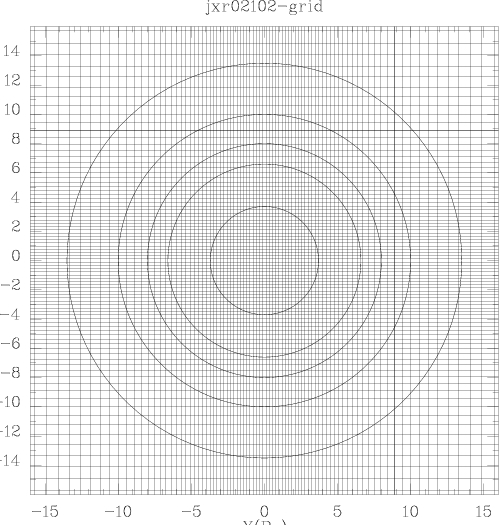
\includegraphics[scale=0.2]{images/StretchedCartesian.jpg}
\begin{itemize}
  \item Grid Choice: Uniform/Stretched Cartesian, SAMR
  \item Boundary/Initial Conditions
  \item Discretization: Finite Differences, Finite Volumes, Finite Elements.
\end{itemize}

\end{frame}

\begin{frame}
\frametitle{Chosen MHD Models}
\begin{tabular}{p{0.4\textwidth}p{0.5\textwidth}}
\centering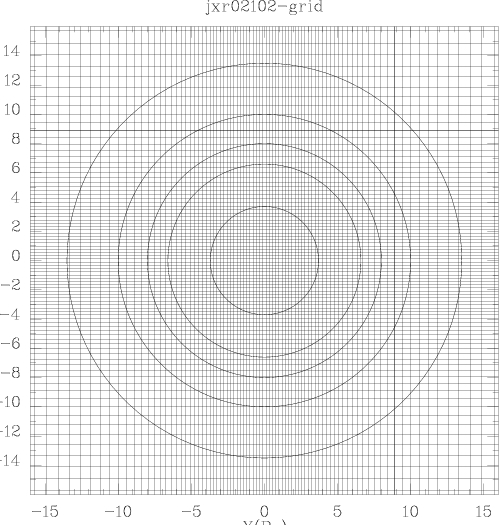
\includegraphics[scale=0.15]{images/StretchedCartesian.jpg}
\begin{itemize}
   \item[] \textbf{OpenGGCM}
   \item Stretched cartesian grid.
   \item Solves resistive MHD. (Not neglecting magnetic diffusivity)
   \item Conservative finite difference.
\end{itemize} &

\centering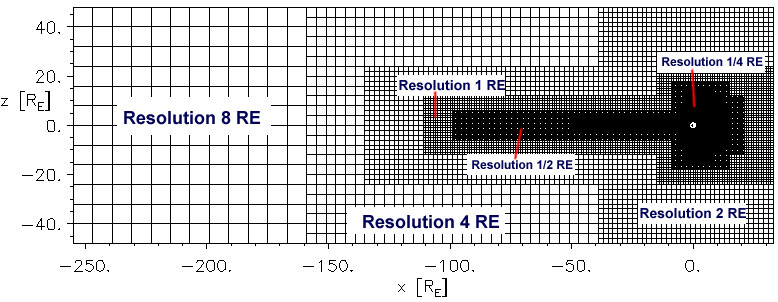
\includegraphics[scale=0.15]{images/BATS-R-US_Grid.jpg}
\begin{itemize}
  \item[] \textbf{BATS-R-US/SWMF}
  \item Block adaptive grid.
  \item Solves ideal MHD.
  \item Finite volumes.
  \item SWMF adds Rice Convection Model.
\end{itemize}
\end{tabular}
\end{frame}